\documentclass{standalone}
\usepackage{tikz}
\usepackage{pgfplots}
\pgfplotsset{compat=newest}
\usepackage{amsmath}
\usepackage[american]{circuitikz}
\usepackage{cmbright}

\definecolor{myred}{RGB}{170,0,0}
\definecolor{myblue}{RGB}{0,0,220}
\definecolor{mygreen}{RGB}{0,150,0}
\definecolor{myorange}{RGB}{255,127,0}
\definecolor{mybrown}{RGB}{150,75,0}

\ctikzset{bipoles/resistor/height=0.2}
\ctikzset{bipoles/resistor/width=0.5}

\begin{document}
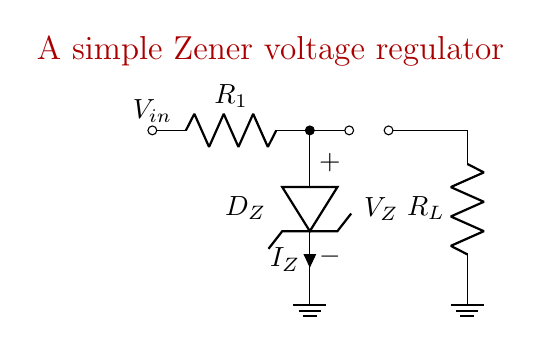
\begin{tikzpicture}
    % A simple voltage regulator.
    \begin{scope}
        \node[anchor=center, color=myred, align=center] at (1.5, 1.0) {\large A simple Zener voltage regulator};
        \node[anchor=center, align=center] at (0, 0.25) {$V_{in}$};
        \draw (0, 0)
            to[R, o-, l={$R_1$}] ++(2.0, 0)
            to[short, *-o] ++(0.5, 0);
        \draw (2.0, 0.0)
            to[zzD, l_={$D_Z$}, v^={$V_Z$}, i_={$I_Z$}] ++(0, -2.0);
        \node[ground] at (2, -1.8) {};
        \draw (3.0, 0.0)
            to[short, o-] ++(1.0, 0)
            to[R, l_={$R_L$}] ++(0, -2.0);
        \node[ground] at (4.0, -1.8) {};
    \end{scope}
\end{tikzpicture}
\end{document}